\documentclass[]{auvsi_doc}
\setkeys{auvsi_doc.cls}{
	AUVSITitle={Design Description},
	AUVSILogoPath={./figs/logo.pdf}
}

% include extra packages, if needed

\begin{document}

\begin{AUVSITitlePage}
\begin{artifacttable}
\entry{DD-001, 0.1, 04-02-19, Initial release, Derek Knowles, Jacob Willis}
\entry{DD-001, 0.2, 04-02-19, Added details, Jacob Willis, Derek Knowles}
\entry{DD-001, 1.0, 04-15-19, No UGV drive key success measures, Jacob Willis, Derek Knowles}
% additional \entry{} commands for extra rows in the revision table, if needed
\end{artifacttable}
\end{AUVSITitlePage}

% document contents (see below for LaTex commands that make your life easier)
\section{Introduction}
A summary of each subteam's design description is provided in the sections below. The subsystems described make up the whole system that will be used at the AUVSI-SUAS 2019 competition. 

\section{Airframe}

The airframe subteam selected the Nimbus Pro airframe.
It is a fixed-wing plane with a large storage capacity and large wing span made of polystyrene (Fig. \ref{fig:plane1}).
It was selected during Concept Development for its long span and spacious fuselage.
Multiple flight tests have been performed with R/C control and the autopilot.
We have also successfully tested system integration with the UGV drop and vision subsystems during flight.
This airframe was selected for its wing span of 1.95 m, total aircraft length of 1.29 m, and internal capacity of approximately 8000 cm\textsuperscript{3}. 
Additionally, it was chosen because by using an off the shelf model we can quickly repair or replace components in the event of crashes or failures.
Some small modifications were made to the plane in order to improve its performance, namely increasing the horizontal stabilizer incidence angle, adding a camera viewport, and creating a payload bay drop door.

\begin{figure}[h!]
	\centering
	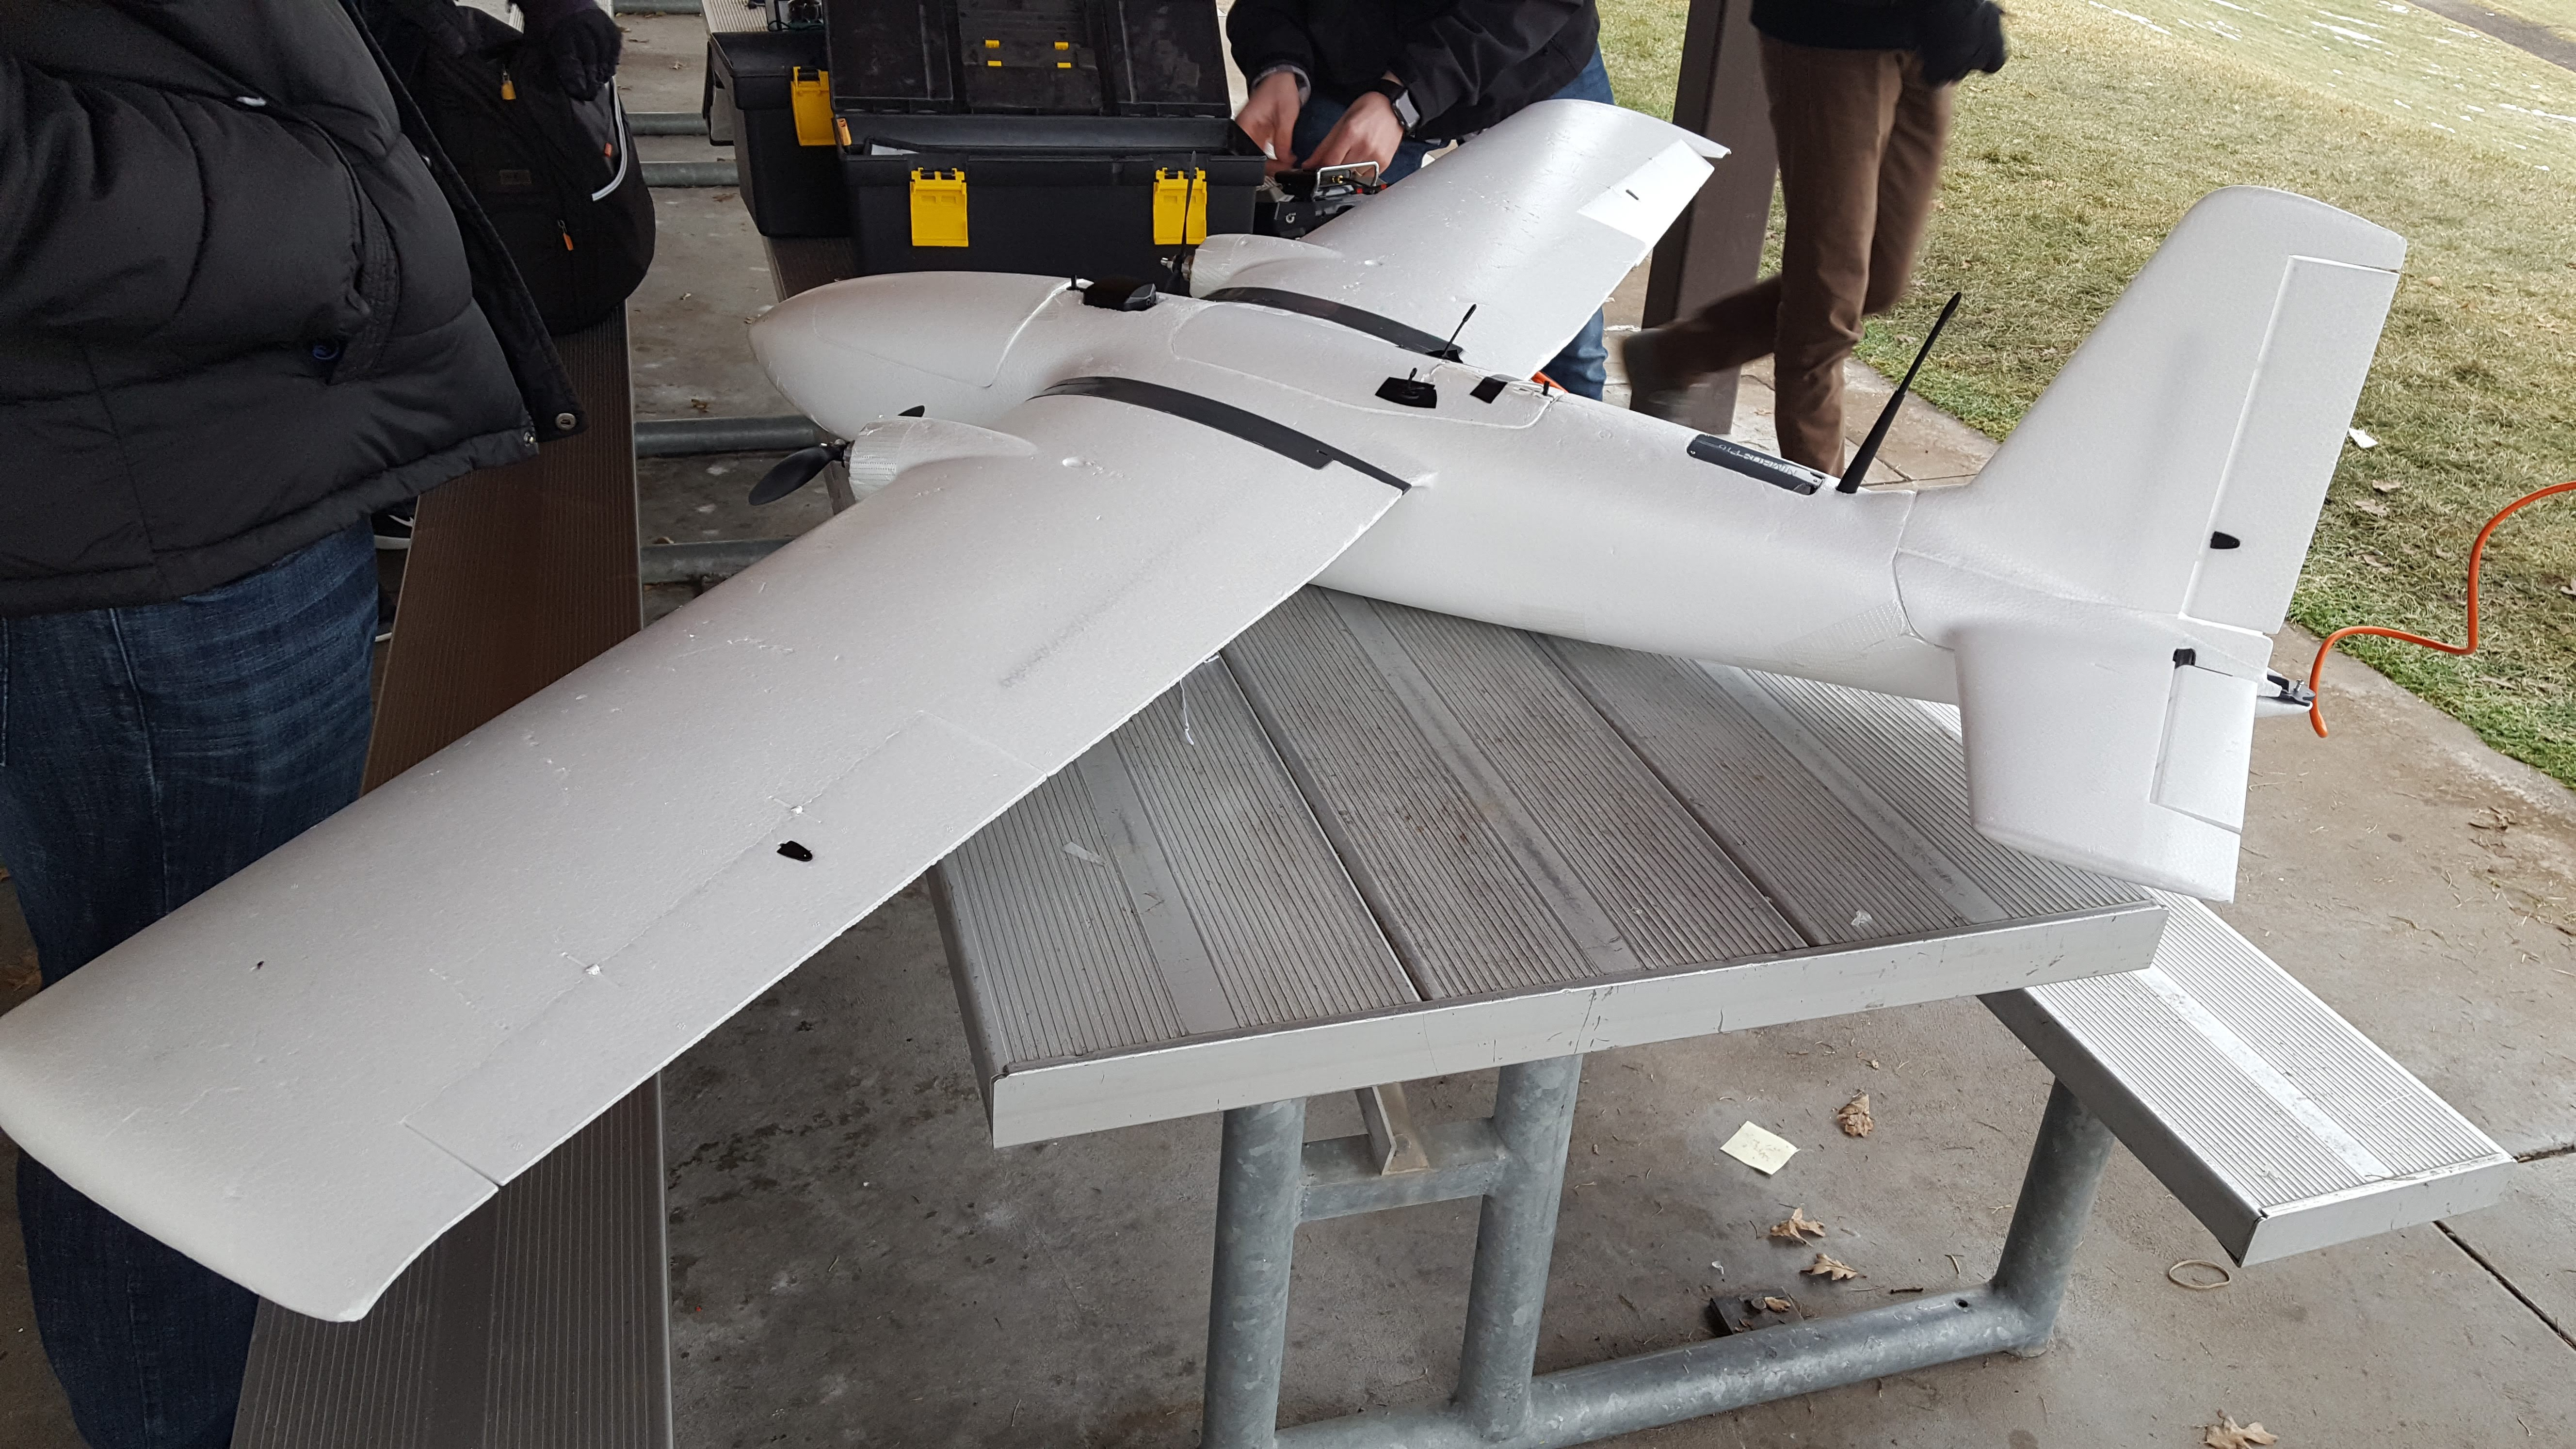
\includegraphics[width=.9\columnwidth]{figs/plane1}
	\caption{Fully-constructed Nimbus Pro airframe before its first flight.}
	\label{fig:plane1}
\end{figure}

\section{Controls}
The purpose of the controls subsystem is to provide the UAS with the ability to autonomously fly waypoints and avoid obstacles.
This subsystem works based on the principles described in Dr. McLain and Dr. Beard's \textit{Small Unmammed Aircraft} book.
Mission objectives are obtained from the judge's server.
A flight path is determined from the objectives using an Rapidly-exploring Random Tree (RRT) method which randomly grows a tree until a path that connects all desired objective points is determined.
Once a path has been determined, the plane attempts to minimize the distance between its planned path and current location through a series of proportional-integral-derivative (PID) controllers that adjust the airplane control surfaces.


\section{Vision}
The main goal of the vision subsystem is to detect, classify, and geolocate ground targets on the competition field using a downward-pointing camera mounted to the airframe. 
This portion of the competition can be done either manually or autonomously, with more points being awarded for autonomously-detected targets.
Our team chose to have a manual detection and classification system running in parallel with an autonomous system to maximize the amount of points awarded. A brief description of the different systems is given below.

In order for points to be awarded for autonomous submissions, there must be no human interference from the time the picture is taken to the time classifications are submitted to the judges. First, raw images are passed to a detector that finds regions of interest (ROIs). These ROIs are then examined to extract images of the target shape and letter, which are then classified by pretrained neural networks. The shape color and letter color are then identified and the classification is submitted to the judges.

The manual detection is performed in a similar manner, but with the identification and classification being done by a human client. This is performed using a GUI which allows up to three clients to work simultaneously, as well as monitor the autonomous submissions. Should the autonomous system register more than 10 false positives during the target detection sequence, a client will shut down the autonomous system, finishing up the target detection portion of the competition manually.
In order to address concerns with the way the past year's team spread image classification
across multiple machines making it difficult to identify bugs, replicate
results and setup quickly, our team created a
basic server-client architecture as defined as shown in Figure \ref{fig:serverFlow}.
The basic data flow of all these components is shown in Figure \ref{fig:dataFlow}.
Data flows back and forth between client and server, with the server holding a definitive-final
copy of a target image, as well as a history of its state during intermediate steps.

\AUVSIFigure
{./figs/serverFlowchart.pdf}
{\textwidth}
{Server Architecture}
{fig:serverFlow}


\AUVSIFigure
{./figs/basicDataFlow.pdf}
{\textwidth}
{AUVSI Imaging Data Flow Through Autonomous/Manual Classification}
{fig:dataFlow}


\section{UGV}

The UGV is a ground vehicle that must be loaded within the aircraft prior to flight, and fly with the aircraft through the waypoint portion of the mission. 
Upon a command from the flight controller system, a small hatch opens and the UGV falls out.
The UGV is carried to the ground by a lightweight 36 inch nylon parachute, purchased from FruityChutes.
The parachute is loaded onto the aircraft in a tube that allows the UGV to pull it out of the aircraft as it falls.
This helps stop the tangling that can come from a folded parachute.
To also prevent tangling, and to make for a more predictable drop, the parachute is folding according to GV-007.
After exiting the aircraft the parachute will be opened by drag.
This will slow down the UGV enough to allow the it to survive impact without damage.
A visual depiction of our chosen system can be seen in Fig.~\ref{fig:side}.

Note that the driving functionality of the unmanned ground vehicle subsystem was considered out of scope for capstone, and there are no key success measures related to it.
As such, there are no capstone documents on driving the UGV.

\begin{figure}[h]
\centering
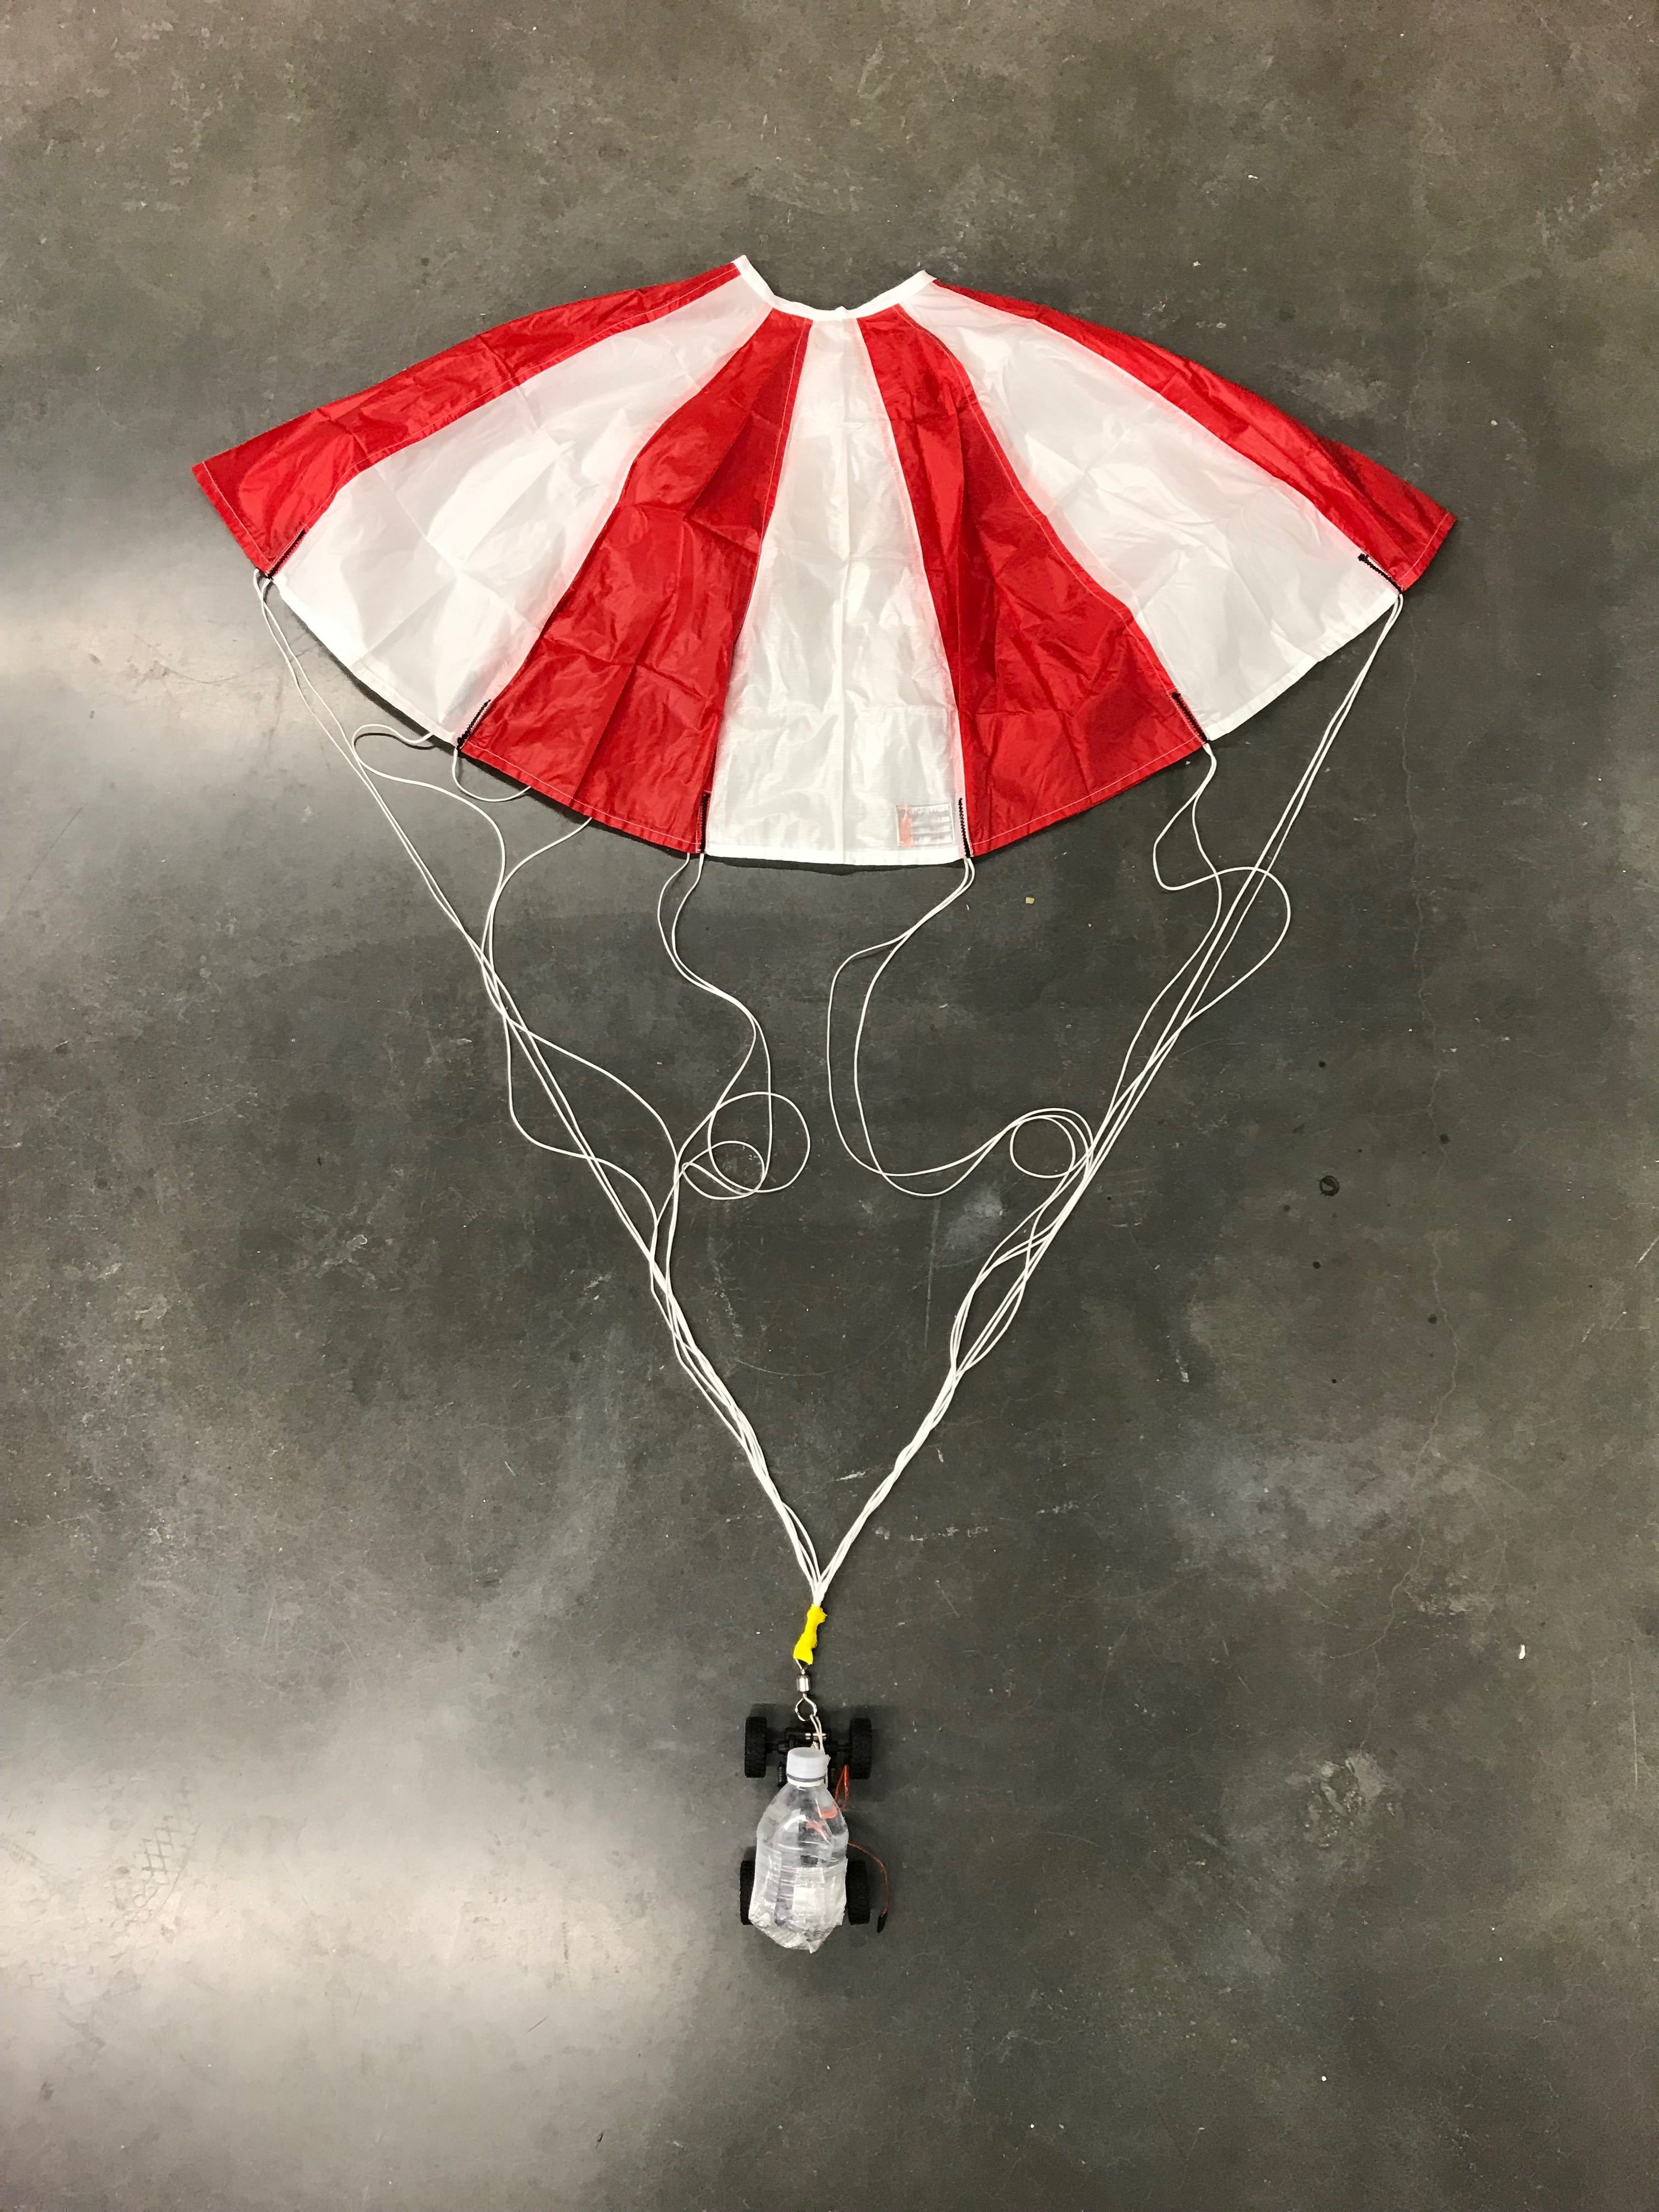
\includegraphics[width=90mm]{./figs/Parachute_Side.jpg}
\caption{Our parachute and simulated UGV as seen from the side.}
\label{fig:side}
\end{figure}

\section{Conclusion}

This year's AUVSI team has increased the desirability and transferability of the Unmanned Aircraft System. Each subteam
has make progress on each of the key success measures thereby increasing the reliability of each subsystem.

\end{document}
